\chapter{More About Configuring MATSim}
\label{ch:configuring}
% ##################################################################################################################

\hfill \textbf{Author:} Andreas Horni, Kai Nagel

\begin{center} 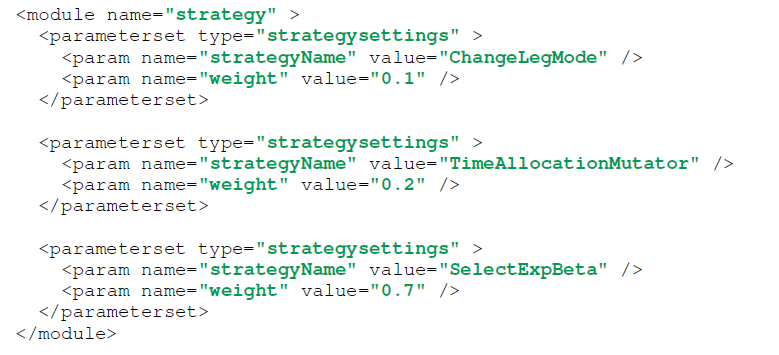
\includegraphics[width=0.3\textwidth, angle=0]{using/figures/strategy.png} \end{center}

% ##################################################################################################################
In this chapter, configuration options are described that can be used together with the tree basic elements \gls{configfile}, population and network.
%are exclusively done by the \gls{configfile}. \gls{matsim} configuring  requiring
%% Aspects that require further input data are described in Chapter~\ref{ch:modules}. The technical details for module usage, in particular the parameter sets are described in \citep[][]{MATSim_Userguide_2015} and in the \gls{javadoc}.
%
Part~\ref{part:extending-matsim} will discuss various options to extend \gls{matsim} beyond these three elements, sometimes by just using additional files, sometimes by using additional \gls{jar} files beyond the \gls{matsim} core \gls{jar} file,  sometimes by writing so-called ``scripts in \gls{java}'', and sometimes by adding or replacing functionality.

\gls{matsim} writes configuration files at several places, for example in the logfile, in the iteration output directory, or the \lstinline{CreateFullConfig} functionality described in Section~\ref{sec:lgs-config}.  As already explained in Section~\ref{sec:survival}, these files come with comments that explain the configuration options.  This is often the best source to understand configuration options.  %\kai{Andreas, meinem Eindruck nach geht der user guide hier auch nicht weiter als das Buch -- und soll es derzeit auch gar nicht.  Unsere Javadoc sagt m.E.\ traditionell sehr wenig bis gar nichts über config.} \ah{ok}

% ##################################################################################################################
\section{MATSim Data Containers}
\label{sec:using-data-containers}
%% \kai{Eigentlich steht das alles schon in Section~\ref{sec:inputdata}.  Ist es wirklich sinnvoll, das zu doppeln?  Oder schreiben wir hier halt die ``weiteren'' Container rein (dann sollten wir aber einiges weitere von oben hier runter holen).}
%% \ah{M.E. jetzt ok.}

% ===================================================================================
\subsection{Network}
\label{sec:using-network}
The \gls{configfile} section \lstinline|network|
%amongst other
specifies which network file will be used in the simulation (Section~\ref{sec:lgs-config} and \ref{sec:lgstarted-network-file}). Further configuration options, \eg specification of time-variant networks, are presented in Section~\ref{sec:extending-network}.

% ===================================================================================
\subsection{Population}
\label{sec:using-population}
The \gls{configfile} section \lstinline|plans| allows to specify the population with its day plans (Section~\ref{sec:lgs-config} and \ref{sec:lgstarted-population-file}). Further configuration options, \eg specification of arbitrary agent attributes or subpopulations, are presented in Section~\ref{sec:extending-population}.

Further \gls{matsim} containers are described in Section~\ref{sec:extending-data-containers}.

%##################################################################################################################
\section{Global Modules and Global Aspects}
\label{sec:using-globalmodules}
% ===================================================================================
\subsection{Controler}
\label{sec:using-controler}
The controler is an indispensable module for running \gls{matsim}, its parameters are set in the \lstinline|controler| \gls{configfile} section. The \gls{matsimrun}'s output directory, its number of iterations, and the ouput interval of plans and events can be specified here. Also, the \gls{mobsim} to be used can be defined (Section~\ref{sec:using-mobsims}). Importantly, the routing algorithm is defined here by using
%
\begin{xml}
<module name="controler" >
    <param name="routingAlgorithmType" value="{Dijkstra | FastDijkstra |
    		AStarLandmarks | FastAStarLandmarks}" />
    [...]
</module>
\end{xml}
%
%In Section~\ref{sec:extending-controler}, the
Possibilities to extend the \lstinline|Controler| functionality is given in %Section~\ref{sec:extending-controler} and % da steht nichts mehr. kai, jan'15
Chapter~\ref{ch:extensionpoints}.

% ===================================================================================
\subsection{Parallel Computing}
\label{sec:using-parallel-computing}

\gls{matsim} uses multi-threading in order to accelerate the computing speeds.  Related configuration parameters can be found in several config modules; they are combined into one section here for convenience.

% ...................................
\paragraph{Global Setting}

The \lstinline{global} section contains
\begin{xml}
<module name="global" >
    <param name="numberOfThreads" value="2" />
    [...]
</module>
\end{xml}
This number is used at several places, most importantly for the innovative strategies, where for example multiple routing requests are distributed to multiple threads.

An advisable starting point is to use the number of available cores.

% ...................................
\paragraph{Parallel Event Handling}
\label{sec:using-paralleleventhandling}

The \gls{configfile} section \lstinline|parallelEventHandling| is used to define the number of threads used for event handling. 
As described in \citet[][]{WaraichEtAl_TechRep_IVT_2009, WaraichEtAl_STRC_2009} the simulation can be substantially speed-up when using multiple threads for the events handling, usually being a bottleneck in \gls{matsim} simulation runs.
% Clearly, the number of threads should correspond with available processor cores.  \kai{Meine Erfahrung ist eine andere, und je nach Maschine kann man das manchmal überauslasten und manchmal sollte man es eher unterauslasten.}  
%% According to our experiences the optimal degree of capacity utilization (threads versus cores) is highly machine-dependent.
%% As mentioned above, the \gls{mobsim} \gls{qsim} is running parallel by default.

%% Being able to speed-up scenarios might become even more important than today, when additional innovation (choice) dimensions are added with large variability in the parameters rendering ensemble runs necessary. % (see Section~\ref{sec:variability}).

% ...................................
\paragraph{Parallel QSim}

The number of threads for the paralle \gls{qsim} (\cf \cite{Dobler_PhDThesis_2013}) can be configured by
\begin{xml}
<module name="qsim" >
    <param name="numberOfThreads" value="10" />
    [...]
</module>
\end{xml}

%\ah{Marcel hatte mal Testreihe mit Identifikation der Laufzeit einzelner Module (QSim, Eventshandling etc.) geplant. Nachfragen, ob schon was vorhanden}

% ...................................
\paragraph{General Recommendations}

Quite generally, computations that use threads are not necessarily faster with more threads. The same holds for \gls{matsim}.  In consequence, some experimentation is necesary for each combination of scenario and hardware.  Here are some recommendations:
\begin{itemize}\styleItemize

\item For the ``global'' number of threads, a good starting point is the number of available cores.

\item It is no longer possible to switch of parallel event handling completely, so setting it to `0' or `null' or `1' presently does exactly the same.  Setting it to values larger than one sometimes leads to performance gains, but they are rarely significant.

\item The most sensitive parameter is for the \gls{qsim}.
  %
  For somewhat older hardware (\eg Apple Macbook Pro from~2010), using all three cores that remained besides the parallel event handling led to negligible performance gains while rendering the machine inutilisable even for normal office tasks.
  %
  For new hardware (\eg Apple Macbook Pro from~2014), using six of the available eight cores for the \gls{qsim} can make the \gls{mobsim} more than a factor of two faster while the machine can still be used for office tasks.
  %
  Experiences with older servers say that one needs to investigate carefully the number of threads for the \gls{mobsim} since using more threads often slows it down \citep{Dobler_PhDThesis_2013}.
  %
  Experiences with new servers are currently not available. 
%% \kai{or are there?  where?} \ah{Gemäss Patrick ist Sergio was am Basteln mit Desktop-Clustern.}
  \item High Performance Computing Clusters are often available to researchers, allowing access to high quality machines with reduced management overhead. Typically, one pays for computation time, either directly or by a loss of priority, by an amount proportional to the reserved resources, that is, the time the job took to finish multiplied by the number of reserved cores. In such a setting, the number of cores used throughout the whole process should thus be stable, to avoid paying for unused resources. A recommendation in this case is thus to set the number of threads for the QSim to the best value $n$ (see above), and then set the ``global'' number of threads to this same $n$, and submit the job requesting $n$ cores.
	  Also note that a low number of threads is almost always better in terms of throughput.
	  In addition, both for calibration and ``what-if'' scenario exploration,
	  one typically needs to run a large number of simulations with different parameters or
	  input data.
	  As total RAM memory is usually not an issue on a cluster,
	  it is thus often more efficient to run simultaneously a large number of simulations
	  with a low number of threads, rather than a low number of simulations with lots of threads.

\end{itemize}

%% \kai{number of threads: nicht unter parallel computing?  Wäre meiner Erfahrung nach tatsächlich hilfreich, die paralellen Aspekte zusammenzufassen.} \ah{\url{https://matsim.atlassian.net/browse/MATSIM-310}} \kai{Ich meinte eigentlich eher, sie ``im Buch'' zusammen zu fassen.  Im code scheint mir das derzeit nicht genügende Priorität zu haben, zumal wir mit dem Buch langsam in die Zielgerade kommen müssen.  Bin mir auch nicht sicher, ob wir das im code wirklich umbauen wollen. }


% ===================================================================================
\subsection{Global}
\label{sec:using-global}
In the \gls{configfile} section \lstinline|global|, the simulation's random seed, the ``global'' number of \gls{java} threads (see above), and the coordinate system (\cf Section~\ref{sec:unitsconventions}) can be defined. 

% ##################################################################################################################
\section{Mobility Simulations}
\label{sec:using-mobsims}
An overview of \gls{matsim} mobility simulations is given in \citet[][]{Dobler_TechRep_IVT_2011}. %See also the presentation of \citet[][]{Rieser_unpub_IVT_2011}.

% ===================================================================================
\subsection{\protect\gls{qsim}}
\label{sec:using-qsim}
The queue-based and time-step based \gls{qsim} \citep[][]{Dobler_TechRep_IVT_2011, Dobler_STRC_2010} is \gls{matsim}'s default \gls{mobsim}. 
Its parameters are set in the \lstinline|qsim| \gls{configfile} section. Prominent parameters are as follows.
\begin{itemize} 

\item
By specifying the parameter \lstinline|numberOfThreads| \gls{qsim} can be run in parallel, see Section~\ref{sec:using-parallel-computing}. 

\item Importantly, this section's parameters \lstinline|flowCapacityFactor| and \lstinline|storageCapacityFactor| need to be set accordingly, when running sample scenarios, \eg for a 10\,\% sample, these factors need to be divided by~10. The \gls{matsim} \gls{gui} (Figure~\ref{fig:matsimgui}) allows to adapt these parameters with the command \lstinline|Tools...Create Sample Population|.

\item
The link dynamics, either \gls{fifo} or passing can be specified by the parameter \lstinline|linkDynamics|. 

\item
Back-propagating gaps (Section~\ref{sec:trafficflowmodel}) are only available in an experimental manner, 
they will be added in the near future and will then be configurable with the parameter \lstinline|trafficDynamics|. 
%% \kai{Das gibt es immer noch nicht wirklich.  Habe jetzt Amit rekrutiert, damit er mir da hoffentlich hilft.}
%% \ah{ok. angepasst}
\end{itemize}

As shown in Section~\ref{sec:using-qsim-multimodal}, \gls{qsim} can handle \gls{multimodal} scenarios. %% \kai{chk}

%% \ah{explizit hinzufügen ist jetzt nicht mehr nötig, weil default, oder?}
%% To invoke \gls{qsim}, the parameter \lstinline|mobsim| of \lstinline|controler| \gls{configfile} section must be set to \lstinline|qsim| and a \lstinline|qsim| \gls{configfile} section must be provided.
%% \kai{ja, qsim ist default.}

% ===================================================================================
\subsection{JDEQSim}
\label{sec:using-jdeqsim}
\gls{jdeqsim} \citep[][]{WaraichEtAl_TechRep_IVT_2009, WaraichEtAl_STRC_2009} was used for project \emph{KTI Frequencies} \citep[][]{BalmerEtAl_ResRep_datapuls_2010}. It is is a \gls{java} reimplementation of \gls{deqsim} \citep[][]{WaraichEtAl_STRC_2009, CharyparEtAl_TRR_2007, CharyparEtAl_TRB_2009} and provides parallel event handling but no parallel simulation \citep[][p.11]{BalmerEtAl_ResRep_datapuls_2010}. Back-propagating gaps (Section~\ref{sec:trafficflowmodel}) are supported. Traffic lights, public transport and within-day replanning are not supported.

To run \gls{jdeqsim} the parameter \lstinline|mobsim| of \lstinline|controler| \gls{configfile} section must be set to \lstinline|JDEQSim| and a \lstinline|jdeqsim| \gls{configfile} section must be provided. 

%%%%%%%%%%%%%%%%%%%%%%%%%%%%%%%%%%%%%%%%%%%%
%##################################################################################################################
\section{Scoring}
\label{sec:using-scoring}
The \gls{configfile} section \lstinline|planCalcScore| specifies the parameters used for scoring agents' plans (Section~\ref{sec:lgs-config}); parameters are explained in detail in Chapter~\ref{ch:scoring}.

%%%%%%%%%%%%%%%%%%%%%%%%%%%%%%%%%%%%%%%%%%%%
%%%%%%%%%%%%%%%%%%%%%%%%%%%%%%%%%%%%%%%%%%%%

%##################################################################################################################
\section{Replanning Strategies}
\label{sec:strategymodules}
%\kai{Habe ``strategy'' ans Ende gezogen, weil ein matsim run so auch tatsächlich losgeht: erst mobsim, dann scoring, dann replanning.  Gibt es Argumente für andere Reihenfolgen?} \ah{nein, super Punkt!}

\subsection{Plans Generation and Removal (Choice Set Generation)}

The replanning strategy modules are the basic innovation modules available in \gls{matsim}. We do not call them \emph{choice} modules although they are involved in people's choice making. The choice process, however, is performed over the iterations with an \emph{implicit} choice set and it is not based on explicit probability function drawing. Usually, innovation modules also do no define their own utility function. This is particularly true for random mutation modules, where best response modules such as destination innovation are closer to the standard procedure of choice modeling but still not full-blown choice models. For a detailed discussion of \gls{matsim} in choice modeling context see Chapter~\ref{ch:discretechoice}.

All strategy modules are called by configuring the strategy module in the configuration file as shown in the following example.
%
\begin{xml}
<module name="strategy" >
	<parameterset type="strategysettings" >
		<param name="strategyName" value="ChangeLegMode" />
		<param name="weight" value="0.1" />
	</parameterset>
	
	<parameterset type="strategysettings" >
		<param name="strategyName" value="TimeAllocationMutator" />
		<param name="weight" value="0.2" />
	</parameterset>
	
	<parameterset type="strategysettings" >
		<param name="strategyName" value="SelectExpBeta" />
		<param name="weight" value="0.7" />
	</parameterset>
</module>
\end{xml}
%
Each module is given a weight which determines the probability by which the course of action represented by the module is taken. The weights of the strategy modules are normalized in case they do not sum to one. In this example, each agent changes his leg mode with probability~0.1, its plan timing with probability 0.2. A strategy module is, in the code, always a combination of a plan selector and zero or more strategy module elements. In the example, the agent chooses a plan from his set of plans according to a logit model with probability~0.7. 

By specifying the parameter \lstinline|subpopulation|, replanning strategies can be applied to distinct sub-populations: \eg
\begin{xml}
	<parameterset type="strategysettings" >
		<param name="strategyName" value="ChangeLegMode" />
		<param name="weight" value="0.1" />
		<param name="subpopulation" value="urbanTravelers"/>
	</parameterset>
\end{xml}

In older versions of the \gls{configfile} you will find following deprecated configuration syntax using numbered strategy modules.
%
%% \begin{xml}
%% <module name="strategy" >
%%     <!-- NOTE: The following is deprecated syntax. -->
%%     <param name="ModuleProbability_1" value="0.1" /> 
%%     <param name="Module_1" value="ChangeLegMode" />
%%     <param name="ModuleProbability_2" value="0.2" />
%%     <param name="Module_2" value="TimeAllocationMutator" />
%%     <param name="ModuleProbability_3" value="0.7" />
%%     <param name="Module_3" value="SelectExpBeta" />
%% </module>
%% \end{xml}
%
%
%% \kai{Hier gibt es eine neue, bessere Syntax.  NB dass wir da gerade noch am ``Verhandeln'' sind!}
%% \ah{angepasst}
%
%% By specifying the parameter \lstinline{ModuleSubpopulation_X}, i.e.,
%% \begin{xml}
%%     <!-- NOTE: The following is deprecated syntax. -->
%%     <param name="ModuleSubpopulation_1" value="externalAgent"/>
%% \end{xml}
%% replanning strategies can be applied to distinct sub-populations.
%
% brauchen wir m.E. nicht. kai, jan'15


Please note, that combining strategy modules that are \glspl{contribution} such as destination innovation and public transport is not straight forward. Combine them with care and contact the mailing list in case you are unsure.

%Combining different modules is not straight-forward in MATSim. This important topic urgently awaits future analysis. To begin with, here, the combination of the strategy modules with public transport is presented in Table \ref{tab:combination}.
%
%% ----------------------------------
%\createtable%
%{Strategy Module Combination}%
%{Strategy Module Combination}%
%{\label{tab:combination}}%
%{%
  %\begin{tabular}[c]{|c|c|c|}
   %\hline
%\textbf{Innovation Dimension}	& \textbf{Default Strategy} & \textbf{Public Transport}\\
%\hline
%time innovation & TimeAllocationMutator &  TransitTimeAllocationMutator\\
%\hline
%route innovation & ReRoute & ReRoute \\
%\hline
%mode innovation & \multirow{2}{*}{ChangeLegMode} & \multirow{2}{*}{TransitChangeLegMode} \\
%(all legs get same mode) &  &  \\
%\hline
%mode innovation & \multirow{2}{*}{ChangeSingleLegMode} & \multirow{2}{*}{TransitChangeSingleLegMode} \\
%(each leg can have a different mode) &  &  \\
%\hline
%mode innovation & \multirow{2}{*}{SubtourModeChoice} & \multirow{2}{*}{TransitSubtourModeChoice} \\
%(subtour-based) &  &  \\
%\hline
%destination innovation & LocationChoice & LocationChoice \\
%\hline
  %\end{tabular}
%}%
%{}

%\kai{Ich meine, dass es diese Transit Sonderformen gar nicht mehr gibt.  ????}
%\ah{habs mal auskommentiert und die Warnung über Contrib-Kombinationen oben hingeschrieben.} 

% ===================================================================================
\subsubsection{Time Innovation}
\label{sec:timechoice}
Time innovation is applied by defining its parameters in the \gls{configfile} section \lstinline|TimeAllocationMutator| and by adding 
%
\begin{xml}
	<param name="strategyName" value="TimeAllocationMutator" />
\end{xml}
%
plus its weight to the strategy modules.

The module shifts activity end times randomly within a configurable range as described by \citet[][]{BalmerEtAl_Timmermans_2005, Raney_PhDThesis_2005, Balmer_unpub_VSP_2004, BalmerEtAl_unpub_EIRASS_2004, BalmerEtAl_unpub_STRC_2004}. %A best-reponse approach to time choice is applied by "Planomat" described in Section~\ref{sec:planomat}.

% ===================================================================================
\subsubsection{Route Innovation}
\label{sec:routechoice}

Route innovation is applied by defining its parameters in the \gls{configfile} section \lstinline|planscalcroute|, by adding 
%
\begin{xml}
	<param name="strategyName" value="ReRoute" />
\end{xml}
%
plus its weight to the strategy modules, and by specifying the routing algorithm in the \lstinline|controler| \gls{configfile} section (Section~\ref{sec:using-controler}).
\gls{matsim} routing is described by \citet[]{LefebvreBalmer_STRC_2007, LefebvreBalmer_TechRep_IVT_2007}. 

%The configuration necessary for public transport is shown in Chapter \ref{ch:pt}.  \kai{Da steht m.E.\ noch nichts in der Richtung.  Aber meiner Erinnerung nach ist auch gar keine Sonderkonfiguration mehr nötig.  Michael Z.?}
%
%\ah{Kann tatsächlich auch keine Sonderkonfiguration (mehr) finden unter \url{http://www.matsim.org/docs/tutorials/transit}. Kann man also wegmachen. Muss zu Config-Param "transitRouter" noch was gesagt werden?}

% ===================================================================================
\subsubsection{Mode Innovation}
\label{sec:modechoice}
Mode innovation is applied by adding 
%
\begin{xml}
	<param name="strategyName" value="{ChangeLegMode | ChangeSingleLegMode | SubtourModeChoice}" />
\end{xml}
%
plus its weight to the strategy modules. In the \gls{configfile} a section with one of the mode innovation strategies need to be added, \ie 
%
\begin{xml}
<module name="{changeLegMode | changeSingleLegMode | subtourModeChoice}" >
    [...]
</module>
\end{xml}
%\kai{obiges hat jetzt 2x ``changeLegMode''.  Kann zwar sein, dass das tatsächlich so ist, aber falls ja, sollten wir explizit sagen, dass das kein Tippfehler ist.} \ah{thx}
%
\lstinline|ChangeLegMode| randomly picks one of the plans of a person and changes its mode of transport. By default, the supported modes are driving a car and using public transport. Only one mode of transport per plan is supported. For using different modes for sub-tours on a single day the \lstinline|SubtourModeChoice| module is required. Optionally, car availability is respected. \lstinline|ChangeSingleLegMode| randomly picks one of the plans of a person and changes the mode of transport of one single leg. The leg is picked randomly. In contrast to \lstinline|ChangeLegMode|, it allows for multiple modes in one plan. By default, the supported modes are driving a car and using public transport. Also, this module is able to (optionally) respect car-availability.

Mode innovation is described by \citet[][]{RieserEtAl_TRR_2009, MeisterEtAl_WCTRS_2010, CiariEtAl_STRC_2008, CiariEtAl_STRC_2007}.

\subsubsection{Plans removal}

The maximum number of plans per agent is configured by the setting 
\begin{xml}
<module name="strategy" >
   <param name="maxAgentPlanMemorySize" value="5" />
   [...]
</module>
\end{xml}
If an agent ends up having more plans than these, \gls{matsim} will start removing plans one by one until the maximum number of plans is reached.  Plans to be removed are selected by the setting configured by
\begin{xml}
<module name="strategy" >
   <param name="planSelectorForRemoval" value="..." />
   [...]
</module>
\end{xml}
Starting with release 0.7.x, the config file comments give possible options.

This option is presently not well investigated, \cf Section~\ref{sec:choicesets}.

---

\kai{wo ist plans removal?} \ah{Steht momentan noch bei den Selectors, wie auch im Code \lstinline|org.matsim.core.replanning.selectors.WorstPlanForRemovalSelector|. Sehe da aber nur worst plan removal.}\kai{Andreas, ich Verstehe Deinen Kommentar nicht.  DefaultPlanStrategiesModule listet sie alle auf.  WorstPlanForRemovalSelctor ist eine Wahlmöglichkeit.}



% ===================================================================================
\subsection{Plan Selection (Choice)}
\label{sec:selectors}
Selectors and their weight are also added to the strategy modules
%
\begin{xml}
	<param name="strategyName" value="KeepLastSelected | BestScore | SelectExpBeta
					ChangeExpBeta | SelectRandom | SelectPathSizeLogit" />
\end{xml}
%
Selectors work as follows:
%
\begin{itemize}\styleItemize
	\item \lstinline|KeepLastSelected| keeps the plan selected in the previous iteration.
	\item \lstinline|BestScore| selects the plan with the highest score of the previous iteration.
	\item \lstinline|SelectExpBeta| performs \gls{mnl} selection between plans. It can be configured by the \lstinline|BrainExpBeta| parameter from the scoring group.
	\item \lstinline|ChangeExpBeta| changes to a different plan with probability dependent on $e^{\Delta_{score}}$, where $\Delta_{score}$ is the score difference between the two plans.
	\item \lstinline|SelectRandom| performs random selection between the plans.
	\item \lstinline|SelectPathSizeLogit| selects an existing plan according to the path size logit described by \citet[][]{FrejingerBierlaire_TransResB_2007}.
\end{itemize}
%
Note, that the \lstinline|BestScore| should be used with care as it is prone to getting stuck with sub-optimal plans. Plans that are rated bad due to a random fluctuation in one single iteration, due to \eg a rare traffic jam, will never be tested again. It is therefore recommended to use this in conjunction with \lstinline|SelectRandom| only.

Besides the selectors for plan modification and execution, in the near future also the plan remover will be available for configuration. Per default, the plan with the lowest score is removed if the agent's memory is full. In line with the requirements of \eg simulated annealing approaches, the removal of candidates will be configurable to be probabilistically dependent on the plan score similar to the selection in \lstinline|SelectExpBeta|. This will reduce the probability to get stuck with sub-optimal plans, that were dominant in earlier iterations.
%\ah{siehe Mail by M. Zilske, August 14 "[Matsim-devel] custom plan selector for removal")}

%##################################################################################################################
\section{Other Modes Than Car}
\label{sec:using-othermodesthancar}

%% \kai{new section, pls check.  Also see in ``available modules''!!} \ah{done}

%% \kai{This new section ends up being quite long.  What to do?  Maybe (again) cut into two pieces: (1) by config; (2) extensions--???}

\ah{I think we should explicitly say something about pt vehicles here?}
\ah{Do we actually have all the vehicular traffic interactions in \gls{qsim}, including pt vehicles. have to check that, sorry}
\kai{I am reasonably sure that it is as follows: pt vehicles operate on same network if cars if everything is configured that way.  ``everything'' means, I think, that the pt routes use links that are at the same time car links.  So it is really a data issue, not a modelling or implementation issue.}
\kai{Habe unten mal noch einen Abschnitt ``modes transporting other modes'' eingefügt.}

The \gls{matsim} software started with car as mode of transport since in many regions where it was used at that time, car was the main mode.  The idea to integrate other modes has, however, always been there.

The following sections describes the current multi-modal capabilities of \gls{matsim}.  The material does not only cover options that can be enabled with config options only, but also gives an overview over multi-modal extensions, described in Part~\ref{part:extending-matsim} of the book.

% ===================================================================================
\subsection{QSim Side}
\label{sec:using-qsim-multimodal}
\subsubsection{Multiple Vehicular Modes on the Same Network}
%% The previous sections modelled modes other than car on separate simulation infrastructures, either by teleportation or on separate, congestion-free networks.  Clearly, this does not longer work once these modes are congested as well.  However, often the separate modes are not individually congested but share the same infrastructure, for example cars and trucks, or bicycles, motorbikes, and cars in India \citep{AgarwalEtcMixedTraffic}.  It thus was investigated how to have different modes interact on the same congested network.

%% \paragraph{Pedestrian simulations} A first step was to replace ``car'' by something else, for example ``pedestrian''.  This was possible by re-interpreting the geometric properties so that the flow and storage capacity constraints of the \gls{matsim} queue model \kai{explained where?} would make sense for pedestrians rather than for cars \cite{somePaperFromGregor} \kai{chk}.  

% ..............................
\paragraph{\enquote{Main Modes}}
%% The above approach fails as soon as more than one vehicle type is involved.  Therefor, 
Recently, the ability to allow multiple modes on the same network was introduced.  It is defined by the \lstinline{qsim} config option of type
\begin{xml}
<module name="qsim">
   <param name="mainMode" value="car,truck,bicycle" />
   [...]
</module>
\end{xml}
This will look at the leg mode in the plan, and if that leg mode corresponds to one of the listed main modes, it will generate a vehicle for that leg and make it enter the network.

% ..............................
\paragraph{PassingQ} 
Once the different mode vehicle types have different maximum speeds, the standard \gls{qsim} is no longer sufficient, since it uses \acrfull{fifo} as the queuing discipline, and thus fast vehicles cannot pass slower vehicles.  Here, the so-called Passing(Vehicle)Q can be used instead.  It replaces the \gls{fifo} sorting criterion, where vehicles are sorted by the sequence in which they arrive on the link, by a sorting according to the so-called earliest link exit time, which is computed from the link enter time and the freespeed travel time.  Now using the minimum of the vehicle and the link maximum speeds, the freespeed travel time can be different between vehicles, and thus fast vehicles can obtain an earlier link exit time even if they enter later than slow vehicles.  Details and resulting fundamental diagrams are given by \cite{AgarwalEtcMixedTraffic}.

This option can be enabled by using
\begin{xml}
<module name="qsim">
   <param name="linkDynamics" value="passingQ" />
   [...]
</module>
\end{xml}
in the \lstinline{qsim} section of the \gls{configfile}.

% ..............................
\paragraph{Different Vehicle Types by Mode}
%The \lstinline|PassingQ| makes no difference as long as all vehicles have the same maximum speed. 
%It is therefore possible to define so-called ``mode vehicles'', \ie a typical vehicle for each mode. 
\ah{was not easy to read. reformulated it. pls check}\kai{ok}
\lstinline|PassingQ| with vehicles of the same maximum speed still corresponds to \gls{fifo}. 
The option to simulate scenarios with \st{equal} different \kai{Andreas, ok?} mode-specific maximum speeds is supported by the possibility to define so-called ``mode vehicles'', \ie by specifying a typical vehicle for each mode.
%
This is discussed \kai{where?}.
%\footnote{%
%  
%\ah{ab hier vielleicht nach Part II + forward pointer?  Dann haben wir wieder Konsistenz.}
%
%\kai{Ja das können wir versuchen.} \ah{ok}
%
%In order to not use the pre-defined default vehicle type for each mode, for the time being it is necessary to write a script-in-\gls{java}. \ah{moved this down}
%For the necessary syntax, see the \lstinline{RunMobsimWithMultipleModeVehiclesExample} under \url{http://matsim.org/javadoc} $\to$ core.  
%We will eventually make this available as a config option; at this time, we are still searching for a software design that makes the QSim both pluggable at multiple levels \emph{and} easy to maintain.
%
%}

In order to not use the same pre-defined default vehicle type for each mode, for the time being it is necessary to write a script-in-\gls{java} as shown in Section~\ref{sec:multimodalsim_qsim}.\footnote{We will eventually make this available as a config option; at this time, we are still searching for a software design that makes the \gls{qsim} both pluggable at multiple levels \emph{and} easy to maintain.}

\ah{Should we say something about this? Is that correct?}
\ah{Passing is all-or-none, \ie either every vehicle type can pass every other type or none can pass none. 
However, in reality, there usually is something between \gls{fifo} and free passing, \eg a bus might not be able to pass a car, although being faster, whereas bikes might always be able to slip by cars. Such more fine-grained rules about passing do not yet exist at the time of writing this book. }
\kai{Hm.  Ist nicht ganz einfach zu beschreiben, was da wirklich passiert.  Habe schon viele Stunden mit dem gemeinsamen Paper mit Amit et al verbracht, und endgültig klar ist es immer noch nicht.  }

% ..............................
\paragraph{Planned Vehicle Id}
Routes, as described in Section~\ref{sec:lgstarted-population-file}, can have a planned vehicle \gls{id} as attribute.  At the same time, all available vehicles need to be described by an additional file.  The QSim will then attempt to use that specific vehicle, including its individual attributes such as maximum speed.  
This is discussed \kai{where?}.


%% It is possible to give each planned route a list of possible vehicle \glspl{id} to be used for this route.  
\ah{I think this is not easy to understand, but yes, the ref will probably clarify this}
\kai{Re-wrote it.}

%------------------------------------------------------------
\subsubsection{So-Called \Gls{teleportation}}
All modes that are \emph{not} registered with the \gls{qsim} as ``main modes'' will be teleported.  That is, the \gls{qsim} will, without problems, process legs such as
\begin{xml}
<leg mode="pedelec" >
   <route type="generic" trav_time="00:14:44" distance="2374" />
</leg>
\end{xml}
The \gls{qsim} will generate a departure event (for events see Section~\ref{sec:outputdata}) after the end of the previous activity, and an arrival event 14\,minutes and 44\,seconds later.  The leg will be recorded with a distance of 2\,374\,meters.  If the distance is not used for the scoring (\cf Chapter~\ref{ch:scoring}), it can be left out from the route as well (which is the situation in most present set-ups).

\subsubsection{Modes Transported by Other Modes}

\kai{Andreas, I added this section, please check}

With modes such as car, bicycle, or in some sense even walk, the travellers are at the same time the drivers, i.e.\ the entities that decide about turns at intersections and arrivals (or not) on links.
%
With modes such as public transit or taxi, this is no longer correct: Here, the traveller boards a vehicle, the vehicle moves around in the network, and, with pt,  the traveller has to make a decision at each stop is if she or he wants to get off or not.  The vehicle, in turn, can be a normal participant of the corresponding traffic system, i.e.\ buses and taxis can operate on the normal road network and be caught in the same congestion as cars and trucks.  
%
This is exactly how it works in the \gls{matsim} QSim: taxis typically operate on the same network as cars; pt vehicles may operate on the same network if their routes are defined such that they use the same links as regular cars.


%------------------------------------------------------------
\subsubsection{Departure Handlers}
\label{sec:departure-handlers}
It is possible to register a separate departure handler for each mode; see Section~\ref{sec:mobsim-extension-point} for the syntax.  There are also pre-configured extensions that use this approach:
%
\begin{itemize}\styleItemize

\item The so-called ``multiModal'' extension moves all modes that are registered with it on separate, congestion-free networks.  This is better than \gls{teleportation} since the vehicles (or pedestrians) have defined positions at each point in time, meaning that they can also re-plan, \eg re-route (see Chapter~\ref{ch:multimodalsim}).

\item The public transit extension moves all modes that are registered with it with specific public transit vehicles (see Chapter~\ref{ch:pt}).

\item The dynamic transport systems extension moves all modes that are registered with it with taxis (see Chapter~\pageref{ch:dts}).

\end{itemize}

% ===================================================================================
\subsection{Routing Side}
The question now is how routes are generated.
%% Clearly, the user can write her or is own router which can either be a full-blown network router (\cf Section~\ref{sec:router-extension-point}), or alternatively some heuristic that comes up with plausible travel times and travel distances.  It is, however, much easier to use the preconfigured options, as follows.

%------------------------------------------------------------
\subsubsection{Network Modes}
\label{sec:network-modes}
The following syntax defines for which modes the router should generate network routes, \ie routes that contain a sequence of links to follow:
\begin{xml}
<module name="planscalcroute" >
   <param name="networkModes" value="car, truck" />
   [...]
</module>
\end{xml}
As of the writing of this text, the router will route all these modes on the ``car'' links of the network.  Note that, per the network file \gls{dtd}, ``car'' is the default mode of each link as long as long as the link's mode field is not explicitly filled.


%% , which is also the interpretation if no mode information is attached to a link \kai{\url{https://matsim.atlassian.net/browse/MATSIM-330}}.  For alternatives, see \kai{where?}.

%% \kai{There is still a problem here in that ``car,bicycle'' or even just ``bicycle'' will (I think) route the bicycles on the car network \emph{even when the network contains bicycle links}.}

%------------------------------------------------------------
\subsubsection{Teleportation ...}
% ..............................
\paragraph{... With Teleported Mode Free Speed Factor}
A config entry such as
\begin{xml}
<module name="planscalcroute" >
   <parameterset type="teleportedModeParameters" >
      <param name="mode" value="pt" />
      <param name="teleportedModeFreespeedFactor" value="2.0" />
      <param name="teleportedModeSpeed" value="null" />
      <param name="beelineDistanceFactor" value="null" />
   </parameterset>
   [...]   
</module>      
\end{xml}
means that if the router encounters a leg with mode pt, it generates a ``teleportation'' route whose travel distance is the same as and whose travel time is twice that of a freespeed car route.

This models public transit with the assumption that it roughly travels along the same routes as a car trip would, but takes twice as long \citep[\cf][]{Reinhold2006Konzeptzurintegrierten}.

% ..............................
\paragraph{... With Teleported Mode Speed}  Setting, in the above, something like
\begin{xml}
      <param name="teleportedModeFreespeedFactor" value="null" />
      <param name="teleportedModeSpeed" value="4.167" />
      <param name="beelineDistanceFactor" value="1.3" />
\end{xml}
will, instead, generate a teleportation route whose travel distance is 1.3\,times the beeline distance, and whose travel time is that distance divided by 4.167\,meters per second.

This is for example useful when the travel times of the teleported mode should not change together with car freespeed travel times as a result of a policy measure, or when the travel times of the teleported mode have nothing to do with car travel times.  A disadvantage is that this approach does not take obstacles such as water or mountain areas into account for the teleported modes.

%------------------------------------------------------------
\subsubsection{Other Routing Options}
It is possible to register separate routers for specific mode.  The syntax for this is discussed in Section~\ref{sec:router-extension-point}.  The pre-configured extensions that were discussed in Section~\ref{sec:departure-handlers}---``multiModal'', public transit, taxis---come with corresponding routers.  

In addition, the so-called ``matrix based pt router'' (Section~\ref{sec:matrix-based-pt-router}) uses a list of transit stops, and a matrix of stop-to-stop travel times and travel distances, and based on this information computes a teleported walk leg to the next stop, a teleported walk leg to the destination stop, and a telported walk leg to the final destination.
%% Again, the teleportation facility of the QSim will execute these teleported legs, with departure and arrival events both at the activity locations and origin and destination stops.

% It is also important to note that, 
The matrix based pt router also serves as an example that, given the teleportation capability of the \gls{qsim}, it is possible to come up with arbitrary algorithms for arbitrary modes as long as they generate (expected) travel times and (expected) travel distances.  As said earlier, the \gls{teleportation} facility of the \gls{qsim} will just use these two attributes at face value.  Although with such an approach neither congestion nor en-route replanning are or can be included, it is nevertheless a flexible approach that allows a fully modular addition of arbitrary modes without having to interact with the \gls{qsim}.

% ===================================================================================
\subsection{Scoring Side}
For all modes that are mentioned in the plans, a corresponding scoring section must exist.  See Section~\ref{sec:mathematical-form} for an approximate example.

% ===================================================================================
\subsection{Network Side}
\ah{not sure if my added section helps, if routing is not working properly. but this is then somehow a bug, right?}\kai{Maybe not a bug, but an incomplete design.  And yes, for that reason I would leave out this network section; for the time being you can get meaning out of this only if you write scripts-in-java or use a pre-configured version (e.g.\ CDs multi-modal).}
To model mode interactions, a fully \gls{multimodal} network, \ie a network that has links being shared by different modes must be provided. 
As shown in Section~\ref{sec:lgstarted-network-file}, specification of link modes is done with the network attribute \lstinline|modes|.

%##################################################################################################################
\section{Observational Modules}
\label{sec:observational}

% ===================================================================================
\subsection{Travel Time Calculator}
\label{sec:ttc}
The routing module, as an example, needs travel time estimations for all links of the network. To keep the computational effort feasible, the travel time estimations need to be aggregated to time bins. The parameters of this aggregation, such as the bin size, can be specified in the configuration file section \lstinline|travelTimeCalculator|.

% ===================================================================================
\subsection{Link Stats}
\label{sec:linkStats}
The \lstinline|linkStats| \gls{configfile} section allows to specify the output interval of simulation statistics of individual links. It is configurable, if the simulated volumes should be written per iteration or averaged over multiple iterations. Link stats are, amongst other, used for the comparison with count values as introduced in Section~\ref{sec:extending-counts}. 

% ##################################################################################################################
% Local Variables:
% mode: latex
% mode: reftex
% mode: visual-line
% TeX-master: "../main"
% comment-padding: 1
% fill-column: 9999
% End: 
